\lecture{5: Conditioning Continued, Law of Total Probability}
\textbf{Key Topics:} Law of total probability, conditional independent events

\subsection*{Lecture Summary}
\begin{itemize}
    \item Law of total probability (LOTP)
    \item Definition of conditional independence
    \item Reinforce the difference between conditional independence and unconditional independence
\end{itemize}

\subsection*{Core Concepts}

\definition{\textbf{Conditional Independece} (\bookref{Ch. 2.5})\\
Events $A$ and $B$ are said to be conditionally independent given $E$ if $P(A \cap B|E) = P(A|E)P(B|E)$.
}

\note{
It is easy to make terrible blunders stemming from confusing independence and conditional independence. Two events can be conditionally independent given $E$, but not independent given $E^c$. Two events can be conditionally independent given $E$, but not independent. Two events can be independent, but not conditionally
independent given $E$.

In particular, $P(A, B) = P(A)P(B)$ does not imply $P(A, B|E) = P(A|E)P(B|E)$; we can’t just insert “given $E$” everywhere, as we did in going from LOTP to LOTP with extra conditioning. This is because LOTP always holds (it is a consequence of the axioms of probability), whereas $P(A, B)$ may or may not equal $P(A)P(B)$, depending on what $A$ and $B$ are.
}

The next few examples illustrate these distinctions. Great care is needed in working with conditional probabilities and conditional independence!

\example{\textbf{Conditional independence given $\bm{E}$ vs. given $\bm{E^c}$}\\
Suppose there are two types of classes: good classes and bad classes. In good classes, if you work hard, you are very likely to get an A. In bad classes, the professor randomly assigns grades to students regardless of their effort. Let $G$ be the event that a class is good, $W$ be the event that you work hard, and $A$ be the event that you receive an A. Then $W$ and $A$ are conditionally independent given $G^c$, but they are not conditionally independent given $G$.
}

\example{\textbf{Conditional independence doesn’t imply independence}\\
Suppose we have chosen either a fair coin or a biased coin with probability 3/4 of Heads, but we do not know which one we have chosen. We flip the coin a number of times. Conditional on choosing
the fair coin, the coin tosses are independent, with each toss having probability 1/2 of Heads. Similarly, conditional on choosing the biased coin, the tosses are independent, each with probability 3/4 of Heads.\\

However, the coin tosses are not unconditionally independent, because if we don’t know which coin we’ve chosen, then observing the sequence of tosses gives us information about whether we have the fair coin or the biased coin in our hand. This in turn helps us to predict the outcomes of future tosses from the same coin.\\

To state this formally, let $F$ be the event that we’ve chosen the fair coin, and let $A_1$ and $A_2$ be the events that the first and second coin tosses land Heads. Conditional on $F$, $A_1$ and $A_2$ are independent, but $A_1$ and $A_2$ are not unconditionally independent because $A_1$ provides information about $A_2$.
}

\example{\textbf{Independence doesn’t imply conditional independence}\\
My friends Alice and Bob are the only two people who ever call me on the phone. Each day, they decide independently whether to call me that day. Let $A$ be the event that Alice calls me next Friday and $B$ be the event that Bob calls me next Friday. Assume $A$ and $B$ are unconditionally independent with $P(A) > 0$ and $P(B) > 0$.\\

However, given that I receive exactly one call next Friday, $A$ and $B$ are no longer independent: the call is from Alice if and only if it is not from Bob. In other words, letting $C$ be the event that I receive exactly one call next Friday, $P(B|C) > 0$ while $P(B|A, C) = 0$, so $A$ and $B$ are not conditionally independent given $C$.
}


\subsection*{Conditional Probability}

\theorem{\textbf{Law of total probability} (\bookref{Ch. 2.3})\\
Let $A_1, \dots, A_n$ be a partition of the sample space $S$ (i.e., the $A_i$ are disjoint events and their union is $S$), with $P(A_i) > 0$ for all $i$. Then
$$
P(B) = \sum^n_{i=1} P(B|A_i)P(A_i).
$$
\textit{Proof.} Because these pieces are disjoint, we can add their probabilities to get $P(B)$:
$$
P(B) = P(B \cap A_1) + P(B \cap A_2) + \cdots + P(B \cap A_n).
$$
But we know that $P(B \cap A_i) = P(B|A_i)P(A_i)$.
\begin{center}
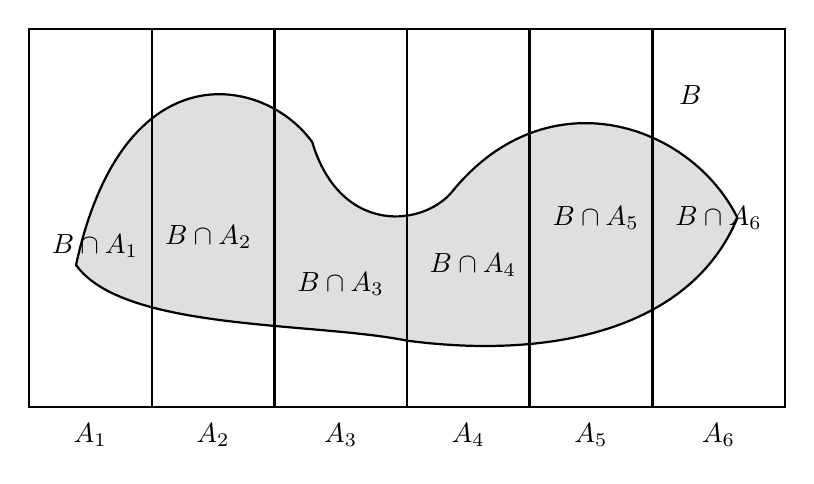
\begin{tikzpicture}[scale=1.2]

% Draw the sample space rectangle
\draw[thick] (0,0) rectangle (8,4);

% Label Ai regions
\node at (0.65,-0.3) {$A_1$};
\node at (1.95,-0.3) {$A_2$};
\node at (3.3,-0.3) {$A_3$};
\node at (4.65,-0.3) {$A_4$};
\node at (5.95,-0.3) {$A_5$};
\node at (7.3,-0.3) {$A_6$};

% Draw event B as an irregular shaded region
\filldraw[fill=gray!25, draw=black, line join=round, thick]
  (0.5,1.5) .. controls (1,3.8) and (2.5,3.5) .. (3,2.8)
  .. controls (3.3,1.8) and (4.2,1.9) .. (4.5,2.3)
  .. controls (5.5,3.5) and (7,3) .. (7.5,2)
  .. controls (7,0.8) and (5.5,0.5) .. (4,0.7)
  .. controls (3,0.9) and (1,0.8) .. (0.5,1.5) -- cycle;

% Draw partitions A1 to A6
\foreach \x in {0,1.3,2.6,4,5.3,6.6,8}
  \draw[thick] (\x,0) -- (\x,4);

% Label B region
\node at (7,3.3) {$B$};

% Label intersections B ∩ Ai
\node at (0.7,1.7) {$B\cap A_1$};
\node at (1.9,1.8) {$B\cap A_2$};
\node at (3.3,1.3) {$B\cap A_3$};
\node at (4.7,1.5) {$B\cap A_4$};
\node at (6.0,2.0) {$B\cap A_5$};
\node at (7.3,2.0) {$B\cap A_6$};

\end{tikzpicture}
\end{center}
}

\example{
A patient named Fred is tested for a
disease called conditionitis, a medical condition that afflicts 1\% of the population. The test result is positive, i.e., the test claims that Fred has the disease. Let D be the event that Fred has the disease and T be the event that he tests positive.

Suppose that the test is “95\% accurate”; there are different measures of the accuracy of a test, but in this problem it is assumed to mean that $P(T|D) = 0.95$ and $P(T^c|D^c) = 0.95$. The quantity $P(T|D)$ is known as the \textit{sensitivity} or \textit{true positive rate} of the test, and $P(T^c|D^c)$ is known as the \textit{specificity} or \textit{true negative rate}.

Find the conditional probability that Fred has conditionitis, given the evidence provided by the test result.

\textit{Solution:} Applying Bayes’ rule and the law of total probability, we have
\begin{align*}
    P(D|T) &= \frac{P(T|D)P(D)}{P(T)}\\
    &= \frac{P(T|D)P(D)}{P(T|D)P(D) + P(T|D^c)P(D^c)}\\
    &\approx 0.16
\end{align*}
}

\theorem{\textbf{Bayes’ rule with extra conditioning} (\bookref{Ch. 2.4})\\
Provided that $P(A \cap E) > 0$ and $P(B \cap E) > 0$, we have
$$
P(A|B, E) = \frac{P(B|A, E)P(A|E)}{P(B|E)}.
$$
}

\theorem{\textbf{LOTP with extra conditioning} (\bookref{Ch. 2.4})\\
Let $A_1, \dots, A_n$ be a partition of $S$. Provided that $P(A_i \cap E) > 0$ for all $i$, we have
$$
P(B|E) = \sum^n_{i=1} P(B|A_i, E) P(A_i|E).
$$
}

The extra conditioning forms of Bayes’ rule and LOTP can be proved similarly to how we verified that $\tilde{P}(A) = P(A|E)$ satisfies the axioms of probability, but they also follow directly from the “metatheorem” that \textit{conditional probabilities are probabilities}.